% !TEX encoding = UTF-8
% !TEX TS-program = pdflatex
% !TEX root = ../tesi.tex

%**************************************************************
\chapter{Descrizione architettura software}
\label{cap:descrizione-architettura}
%**************************************************************

\intro{In questo capitolo verrà descritta l'architettura software del gestionale SAP e dei moduli aggiunti dall'azienda}\\
%**************************************************************
\begin{figure}[!h] 
	\centering 
	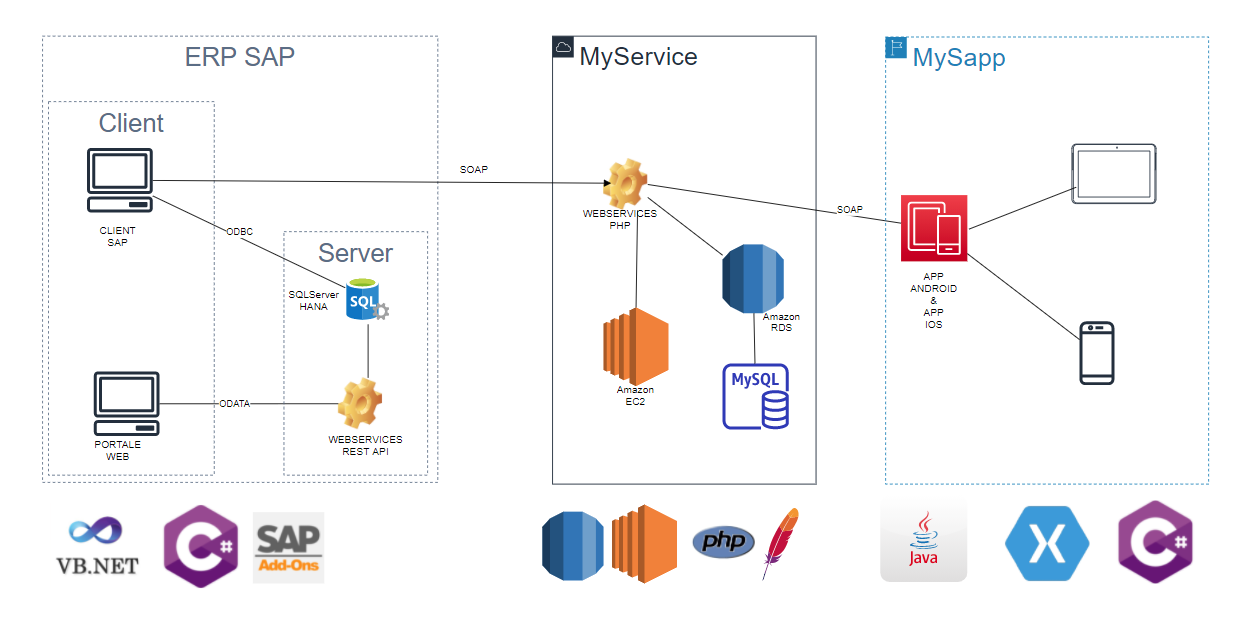
\includegraphics[scale = 0.45]{immagini/architettura-globale.png} 
\end{figure}\\
Da quest'immagine possiamo notare i tre moduli principali:
\begin{itemize}
	\item {ERP SAP:} il modulo del gestionale;
	\item {MyService:} il modulo dei webservices AWS;
	\item {MySapp:} il modulo delle applicazioni Android e iOS.\\
\end{itemize}
Sulle due parti evidenziate dal cerchio rosso si è basato il mio lavoro in questo stage.
Nel client SAP verrà applicato l'applicazione add-on, mentre nei webservices php sono state effettuate delle modifiche ad alcune funzioni.
\section{Descrizione modulo ERP SAP}
\begin{figure}[!h] 
	\centering 
	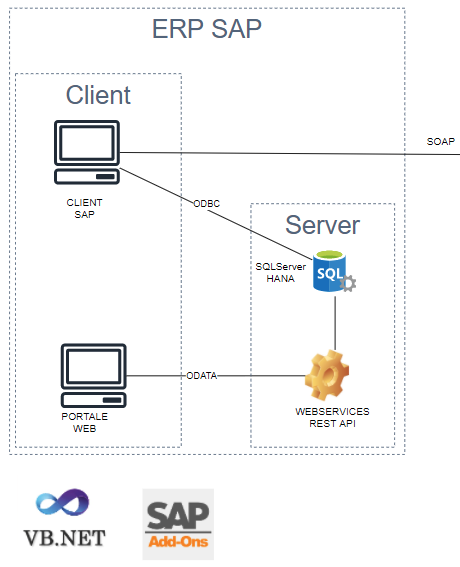
\includegraphics[scale = 0.9]{immagini/modulo-sap.png} 
\end{figure}
\begin{flushleft}
	\item Come possiamo vedere da quest' immagine, il SAP è suddiviso in client e server.\\
	\item Il server può essere basato su :
	\begin{itemize}
		\item SQLServer: solo su Windows;
		\item HANA: solo su Linux.
	\end{itemize}
	\item Il client SAP attualmente è disponibile solo su Windows.\\Sul client SAP possono essere applicati degli add-on, per modificare i comportamenti della GUI del client in base a com'è programmato l'add-on.
\end{flushleft}

\pagebreak 

\subsection{Client SAP}
\begin{flushleft}
	\item Il client SAP utilizza ODBC (open database connectivity) per comunicare con il server SAP.
\end{flushleft}
\begin{figure}[!h] 
	\centering 
	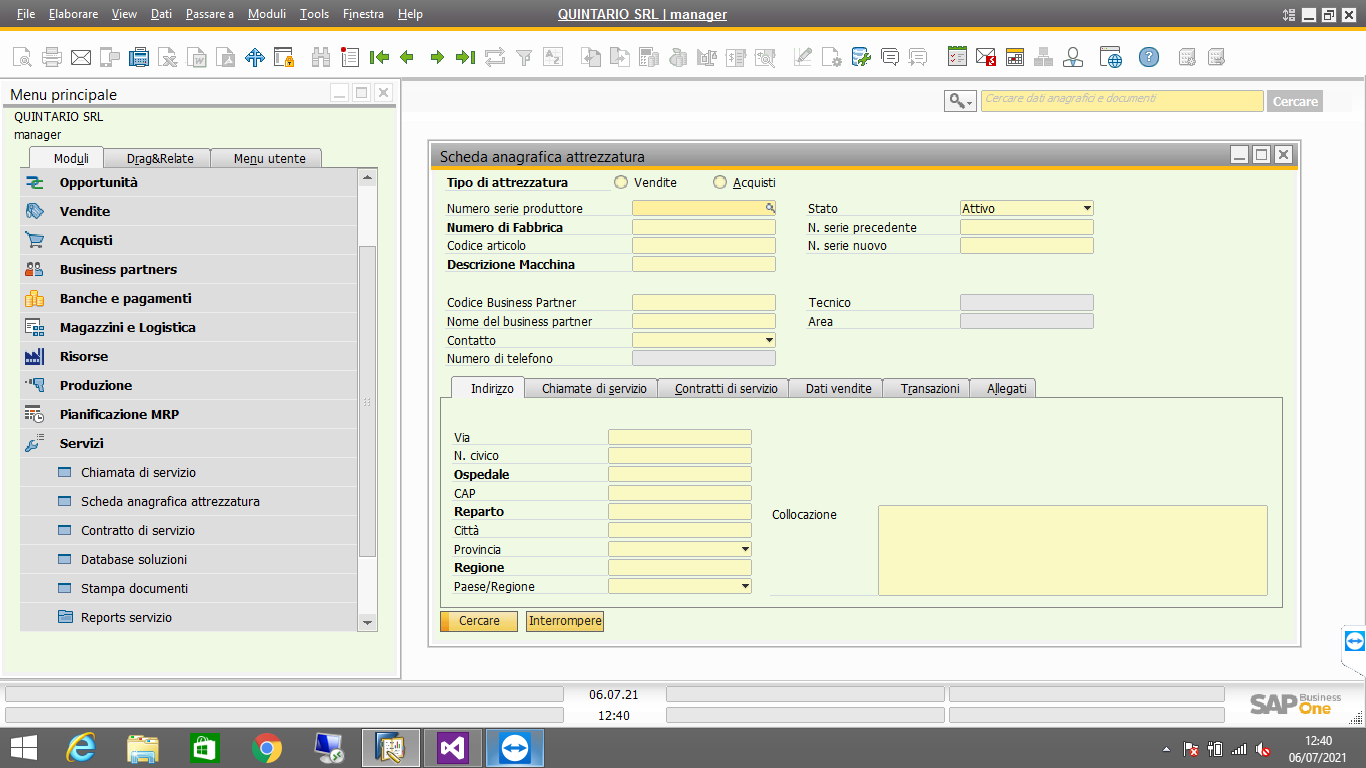
\includegraphics[scale = 0.4]{immagini/client-sap.png} 
	\caption {Client SAP, aperto sulla scheda "Scheda anagrafica attrezzatura"}
\end{figure}
\begin{flushleft}
	\item Qui possiamo vedere come appare il Client SAP, in questo caso è stata aperta la Scheda anagrafica attrezzatura, del modulo dei Servizi.\\Da notare che questi "moduli" del SAP, differiscono dai moduli coinvolti con il modulo del gestionale (MyService e MySapp), questi sono moduli interni del SAP.
	\item La scheda anagrafica attrezzatura è una scheda che rappresenta le attrezzature dell'azienda, ad esempio macchine a controllo numerico, lavatrici o condizionatori, e tutti i possibili macchinari dell'azienda.
	\item Ora vediamo un esempio di cambiamento della GUI di questo client con l'applicazione di un Add-On alla scheda anagrafica attrezzatura.
\end{flushleft}
\pagebreak
\begin{figure}[!h] 
	\centering 
	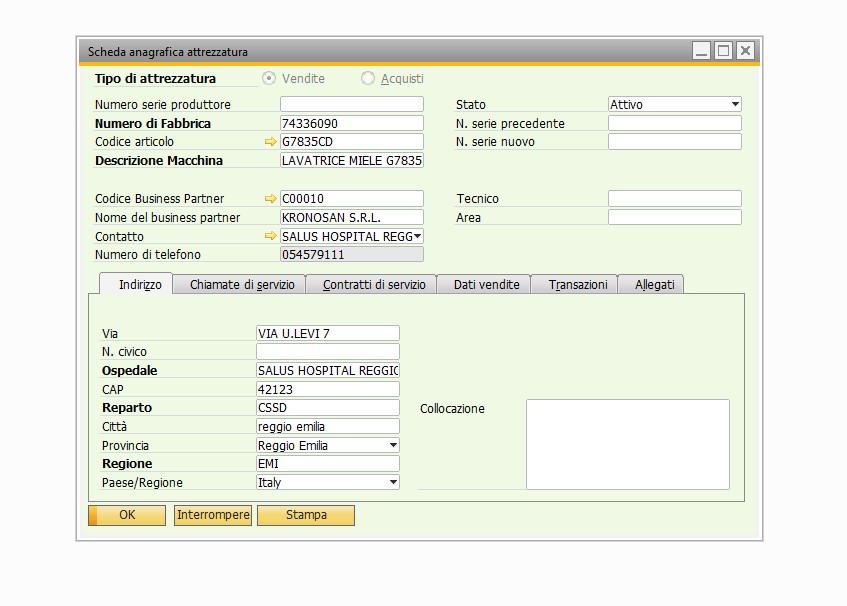
\includegraphics[scale = 0.6]{immagini/esempio-modifica-client-addon.jpg} 
	\caption {Client SAP, esempio di modifica GUI di un add-on applicato sulla scheda "Scheda anagrafica attrezzatura"}
\end{figure}
\begin{flushleft}
	\item Come possiamo vedere è apparso un nuovo pulsante, che stamperà i dati della scheda.\\Questo è un'esempio molto semplice, ma si possono cambiare altre cose, ad esempio aggiungere o rimuovere campi, o aggiungere funzioni ad eventi, ad esempio messaggi di testo che appaiono cliccando dei campi particolari.
\end{flushleft}

\subsection{Portale Web}


\subsection{Webservices REST API}
\begin{flushleft}
	\item Recentemente, su SAP Business One è stato introdotto un service layer, composto da webservices REST API, che comunicano tramite protocollo ODATA (open data protocol).
	\item Questi webservices permettono di accedere direttamente agli oggetti SAP,\\senza passare per il client SAP.\\Gli oggetti SAP sono una struttura dati generata dalla logica del server SAP, \\che raggruppano e ordinano secondo certe logiche i dati presenti nel database.
	\item Per poter ottenere questi dati bisogna fare una richiesta http al webserver, il quale invierà un file json con gli oggetti SAP richiesti.
	\item L'utilizzo più comune di questi webservices è un portale web che usi le informazioni prese tramite queste richiete HTTP. 
\end{flushleft}
\begin{figure}[!h] 
	\centering 
	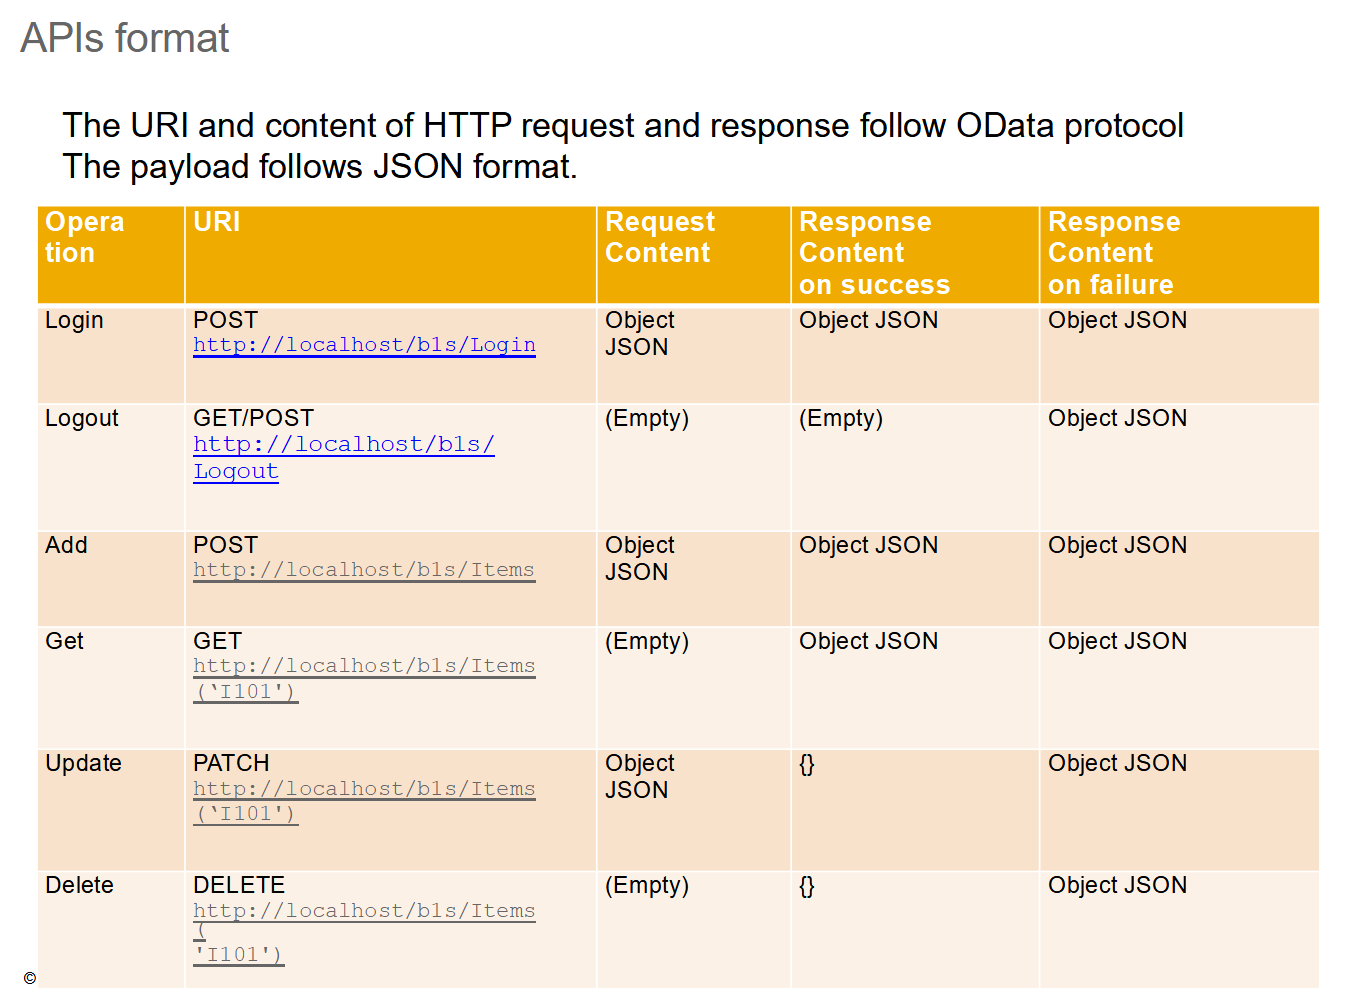
\includegraphics[scale = 0.4]{immagini/api_Format.png} 
	\caption {Formato delle richieste HTTP per il Service Layer SAP}
\end{figure}
\begin{flushleft}
	\item Come si può osservare da quest'immagine, sono presenti le richieste HTTP principali per interagire con i webservices REST API del Service Layer di SAP.
	\item A seguito di una richiesta HTTP viene elaborata la richiesta.\\Viene restituito un oggetto JSON in caso di fallimento, comunicando l'errore causante il fallimento.\\In caso di successo viene restituito un oggetto JSON, ove necessario, oppure un messaggio vuote che rappresenta il successo dell'operazione.
\end{flushleft}



